\documentclass[C++.tex]{subfiles}
\begin{document}

\section{C++17}
\subsection*{Présentation}
\begin{frame}
	\frametitle{Présentation}
	\begin{itemize}
		\item Approuvé en décembre 2017
		\item Dernier Working Draft : \href{http://www.open-std.org/jtc1/sc22/wg21/docs/papers/2017/n4659.pdf}{N4659}
		\item Bon support par CLang 4, GCC 8 et Visual C++ 2017
		\item Progression très rapide du support en parallèle de la normalisation
	\end{itemize}

	\begin{block}{Note}
		Voir \href{https://www.youtube.com/user/lefticus1/videos}{Vidéos C++ Weekly} (Jason Turner)
	\end{block}
\end{frame}

\subsection*{Suppression}
\begin{frame}[fragile]
	\frametitle{Fonctionnalités supprimées}
	\begin{itemize}
		\item Suppression des trigraphes (non dépréciés)
	\end{itemize}

	\begin{block}{Note}
		Les digraphes ne sont pas concernés pour l'instant
	\end{block}

	\begin{itemize}
		\item Suppression de \lstinline|register| (qui reste un mot réservé)
		\item Suppression des opérateurs d'incrément sur les booléens

\note[item]{operator++ déjà déprécié en C++98}

		\item Suppression de \lstinline|std::auto_ptr|
		\item Suppression de \lstinline|std::random_shuffle()|
		\item Suppression des anciens mécanismes fonctionnels : \lstinline|std::bind1st()|, \lstinline|std::bind2nd()|, \ldots
		\item Suppression des spécifications d'exception
	\end{itemize}
		
\note[item]{Mais les fonctions ne levant pas d'exception peuvent être marquées \lstinline|noexcept()|}
\end{frame}

\subsection*{include}
\begin{frame}[fragile]
	\frametitle{Disponibilité des en-têtes : \lstinline|__has_include|}
	\begin{itemize}
		\item Permet de savoir si un fichier d'en-tête est présent \ldots
		\item \ldots{}et donc si une fonctionnalité est disponible
	\end{itemize}

	\begin{lstlisting}[language=C++]
#if __has_include(<optional>)
#  include <optional>
#  define OPT_ENABLE
#endif\end{lstlisting}
\end{frame}

\subsection*{inline variable}
\begin{frame}[fragile]
	\frametitle{\textit{inline variable}}
	\begin{itemize}
		\item Sémantique \lstinline|inline| identique sur fonctions et variables
		\item Peut être définie, à l'identique, dans plusieurs unité de compilation
		\item Se comporte comme s'il n'y avait qu'une variable
	\end{itemize}

	\begin{lstlisting}[language=C++]
inline int foo = 42;\end{lstlisting}

	\begin{itemize}
		\item \lstinline|constexpr| sur une donnée membre statique implique \lstinline|inline|
		\item Utile pour initialiser des variables membres statiques non constantes
	\end{itemize}

	\begin{lstlisting}[language=C++]
class Foo { static inline int bar = 42;};\end{lstlisting}

	\begin{alertblock}{Don't}
		Pas une justification aux variables globales
	\end{alertblock}
\end{frame}

\subsection*{Namespace}
\begin{frame}[fragile]
	\frametitle{\textit{Nested namespace}}
	\begin{itemize}
		\item Nouvelle manière de définir des imbrications de namespaces via l'opérateur \lstinline|::| 
	\end{itemize}

	\begin{lstlisting}[language=C++]
namespace A {
namespace B {
namespace C {
...
}}}

// Devient

namespace A::B::C {
...
}\end{lstlisting}
\end{frame}

\subsection*{static\_assert}
\begin{frame}[fragile]
	\frametitle{\lstinline|static_assert| sans message}
	\begin{itemize}
		\item \lstinline|static_assert| sans message utilisateur
	\end{itemize}

	\begin{lstlisting}[language=C++]
static_assert(sizeof(int) == 3);
// Erreur de compilation\end{lstlisting}
\end{frame}

\subsection*{if constexpr}
\begin{frame}[fragile]
	\frametitle{\lstinline|if constexpr|\titlehfill{}1/4}
	\begin{itemize}
		\item Branchement évalué à la compilation (\textit{static-if})
	\end{itemize}

	\begin{lstlisting}[language=C++]
if constexpr(cond)
  statement1;
else if constexpr(cond)
  statement2;
else
  statement3;\end{lstlisting}

	\begin{itemize}
		\item Conditions d'arrêt plus simple avec les \textit{variadic template}
		\item Moins de spécialisations explicites

\note[item]{Plus besoin d'avoir une spécialisation \og zéro-paramètre\fg{}}
	\end{itemize}

	\begin{block}{Note}
		Conditions intégralement évaluables au \textit{compile-time}, pas de court-circuit

\note[item]{C'est à dire qu'en cas de condition composée (or, and), même si la première partie permet de résoudre la condition, il faut que le reste soit évaluable en \textit{compile-time}}
	\end{block}
\end{frame}

\begin{frame}[fragile]
	\frametitle{\lstinline|if constexpr|\titlehfill{}2/4}
	\begin{lstlisting}[language=C++]
template <typename T> auto foo(T t) {
if constexpr(is_pointer_v<T>)
  return *t;
else
  return t;}

int a = 10, b = 5;
int* ptr = &b;
cout << foo(a) << ' ' << foo(ptr);  // 10 5\end{lstlisting}
\end{frame}

\begin{frame}[fragile]
	\frametitle{\lstinline|if constexpr|\titlehfill{}3/4}
	\begin{block}{Note}
		Les deux branches doivent être syntaxiquement correctes mais pas nécessairement sémantiquement valides
	\end{block}

	\begin{block}{Note}
		Les deux branches peuvent avoir des types retour différents sans remettre en cause la déduction de type retour
	\end{block}

	\begin{exampleblock}{Do}
		Remplace avantageusement certaines constructions basées sur une suite de spécialisations de template et SFINAE, une imbrication illisible d'opérateur ternaire ou l'utilisation de \lstinline|#if|
	\end{exampleblock}
\end{frame}

\begin{frame}[fragile]
	\frametitle{\lstinline|if constexpr|\titlehfill{}4/4}
	\begin{block}{Le \textit{hello world} de la récursion}
		\begin{lstlisting}[language=C++]
template<int  N>
constexpr int fibo(){ return fibo<N-1>()+fibo<N-2>(); }
template<>
constexpr int fibo<1>() { return 1; }
template<>
constexpr int fibo<0>() { return 0; }

// Devient

template<int N>
constexpr int fibo() {
  if constexpr (N>=2) return fibo<N-1>()+fibo<N-2>();
  else return N; }\end{lstlisting}
	\end{block}
\end{frame}

\subsection*{if(init; condition) and switch(init; condition)}
\begin{frame}[fragile]
	\frametitle{\textit{if init statement}\titlehfill{}1/2}
	\begin{itemize}
		\item Initialisation dans le branchement
		\item Portée identique aux déclarations dans la condition
	\end{itemize}

	\begin{lstlisting}[language=C++]
if(int foo = 42; bar)   cout << foo;
else                    cout << -foo;\end{lstlisting}

	\begin{itemize}
		\item Sémantiquement équivalent à
	\end{itemize}

	\begin{lstlisting}[language=C++]
{
  int foo = 42;
  if(bar)  cout << foo;
  else     cout << -foo;
}\end{lstlisting}
\end{frame}

\begin{frame}[fragile]
	\frametitle{\textit{if init statement}\titlehfill{}2/2}
	\begin{itemize}
		\item Alternative intéressante à certaines constructions peu lisibles
	\end{itemize}

	\begin{lstlisting}[language=C++]
if((bool ret = foo()) == true) ...\end{lstlisting}

	\begin{itemize}
		\item \ldots{} ou injectant un symbole inutile au delà du branchement
	\end{itemize}

	\begin{lstlisting}[language=C++]
bool ret = foo();
if(ret) ...\end{lstlisting}

	\begin{itemize}
		\item \ldots{} ou nécessitant l'introduction d'une portée supplémentaire
	\end{itemize}

	\begin{lstlisting}[language=C++]
{
  bool ret = foo();
  if(ret) ...
}\end{lstlisting}
\end{frame}

\begin{frame}[fragile]
	\frametitle{\textit{switch init statement}}
	\begin{itemize}
		\item Pendant du \textit{if init statement}
		\item Initialisation dans le \lstinline|switch()|
		\item Utilisable dans le corps du \lstinline|switch()|
	\end{itemize}

	\begin{lstlisting}[language=C++]
switch(int foo = 42; bar) {
  case ...
}\end{lstlisting}
\end{frame}

\subsection*{structured binding}
\begin{frame}[fragile]
	\frametitle{\textit{structured binding}\titlehfill{}1/5}
	\begin{itemize}
		\item Décompose automatiquement des types composés en de multiples variables

		\begin{lstlisting}[language=C++]
auto [liste de nom] = expression;\end{lstlisting}

		\item Sur des types dont les données membres non statiques
		\begin{itemize}
			\item Sont toutes publiques
			\item Sont toutes des membres directs du type ou de la même classe de base publique
			\item Ne sont pas des unions anonymes
		\end{itemize}

		\item Et sur les classes implémentant \lstinline|get<>()|, \lstinline|tuple_size| et \lstinline|tuple_element|	
		
		\item Notamment : 
		\begin{itemize}
			\item \lstinline|std::tuple|
			\item \lstinline|std::pair|
			\item \lstinline|std::array|
			\item tableaux C
		\end{itemize}
	\end{itemize}
\end{frame}

\begin{frame}[fragile]
	\frametitle{\textit{structured binding}\titlehfill{}2/5}
	\begin{lstlisting}[language=C++]
tuple<int, long, string> foo();
auto [x,y,z] = foo();\end{lstlisting}

	\begin{lstlisting}[language=C++]
class Foo {
  const int i = 42;
  const string s{"Hello"}; 
  public: template <int N> auto& get() const {
    if constexpr(N == 0) { return i; }
    else { return s; } } };
template<> struct tuple_size<Foo>
  : integral_constant<size_t, 2> {};
template<size_t N> struct tuple_element<N, Foo> {
  using type = decltype(declval<Foo>().get<N>()); };

auto [ i, s ] = Foo{};\end{lstlisting}

\note[item]{Les définitions de \lstinline|tuple_size| et \lstinline|tuple_element| sont dans \lstinline|std|}
\end{frame}

\begin{frame}[fragile]
	\frametitle{\textit{structured binding}\titlehfill{}3/5}
	\begin{itemize}
		\item Compatible avec \lstinline|const|

		\begin{lstlisting}[language=C++]
tuple<int, long, string> foo();
const auto [x,y,z] = foo();\end{lstlisting}

		\item \ldots{}avec les références

		\begin{lstlisting}[language=C++]
auto& [refX,refY,refZ] = monTuple;\end{lstlisting}
	\end{itemize}

	\begin{alertblock}{Attention}
		La portée de l'objet référencé doit être supérieure à celle des références
	\end{alertblock}

\end{frame}

\begin{frame}[fragile]
	\frametitle{\textit{structured binding}\titlehfill{}4/5}
	\begin{itemize}
		\item \ldots{}avec \textit{range-based for loop}

		\begin{lstlisting}[language=C++]
map<int, string> myMap;    
for(const auto& [k,v] : myMap) 
{ ... } \end{lstlisting}

		\item \ldots{}avec \textit{if init statement}

		\begin{lstlisting}[language=C++]
if(auto [iter, succeeded] = myMap.insert(value); succeeded)
{ ... }\end{lstlisting}
	\end{itemize}
\end{frame}

\begin{frame}[fragile]
	\frametitle{\textit{structured binding}\titlehfill{}5/5}
	\begin{block}{Objectif}
		Meilleure lisibilité\\
		Remplace des usage de \lstinline|std::tie()|
	\end{block}

	\begin{block}{Nom}
		Appelé déstructuration (\textit{destructuring}) dans d'autres langage
	\end{block}

	\begin{block}{Et ensuite ?}
		Un premier pas vers les types algébriques de données et le \textit{pattern matching}
	\end{block}

\note[item]{Type algébrique : type somme de types produit}
\note[item]{Type produit : analogue sur les types du produit cartésien sur les ensembles}
\note[item]{Type somme : analogue sur les types de l'union disjointe}

	\begin{alertblock}{Limite}
		Pas de capture de \textit{structured binding} par les lambdas
	\end{alertblock}

\note[item]{Possible de passer par la capture généralisée}

\end{frame}

\subsection*{Ordre d'évaluation}
\begin{frame}[fragile]
	\frametitle{Ordre d'évaluation}
	\begin{itemize}
		\item Ordre d'évaluation fixé
		\begin{itemize}
			\item De gauche à droite pour les expressions post-fixées

\note[item]{donc fonction avant paramètre, classe/structure avant membre, tableau avant indice}

			\item De droite à gauche pour les affectations
			\item De gauche à droite pour les décalages
		\end{itemize}
	\end{itemize}
\end{frame}

\subsection*{Copy elision}
\begin{frame}[fragile]
	\frametitle{Élision de copie garantie\titlehfill{}1/2}
	\begin{itemize}
		\item Élision de copie garantie pour les objets créés dans l'instruction de retour
	\end{itemize}

	\begin{lstlisting}[language=C++]
T f() {
  return T{}; } // Pas de copie\end{lstlisting}

	\begin{lstlisting}[language=C++]
T g() {
  T t;
  return t; }   // Copie potentielle eludee\end{lstlisting}
\end{frame}

\begin{frame}[fragile]
	\frametitle{Élision de copie garantie\titlehfill{}2/2}

	\begin{itemize}
		\item Élision de copie garantie  lors de l'initialisation de la définition d'une variable locale
	\end{itemize}

	\begin{lstlisting}[language=C++]
T t = f();   // Pas de copie\end{lstlisting}

	\begin{itemize}
		\item Même en l'absence de constructeur par copie
	\end{itemize}

	\begin{block}{Note}
		Élision de copies possibles avant C++17, garanties maintenant
	\end{block}
\end{frame}

\subsection*{Initialisation}
\begin{frame}[fragile]
	\frametitle{\textit{Aggregate Initialisation}}
	\begin{itemize}
		\item Généralisation aux classes dérivées
		\item Incluant l'initialisation de la classe de base
	\end{itemize}

	\begin{lstlisting}[language=C++]
struct Foo {int i;};
struct Bar : Foo {double l;};

Bar bar{{42}, 1.25};
Bar baz{{}, 1.25};   // Foo non intialise\end{lstlisting}

	\begin{alertblock}{Attention}
		\begin{itemize}
			\item Uniquement sur de l'héritage public et non virtuel
			\item Pas de constructeur fourni par l'utilisateur (y compris hérité)
			\item Pas de donnée membre non statique privée ou protégée
			\item Pas de fonction virtuelle
		\end{itemize}
	\end{alertblock}

\note[item]{Bref les autres restrictions continuent de s'appliquer}
\note[item]{Pour résumer, C++14 a levé l'interdiction de membres initialisés par défaut, et C++17 assoupli celle sur \og pas d'héritage\fg{}}
\end{frame}

\begin{frame}[fragile]
	\frametitle{Déduction de type et \textit{Initializer list}}
	\begin{itemize}
		\item Évolution des règles de déduction sur les liste entre accolade
		\begin{itemize}
			\item \textit{Direct initialisation} : déduction d'une valeur
			
\note[item]{S'il y a une unique valeur. C'est une erreur sinon}
			
			\item \textit{Copy initialisation} : déduction d'un \lstinline|initializer_list|
			
\note[item]{Si tous les éléments sont du même type. C'est une erreur sinon}
		\end{itemize}
	\end{itemize}

	\begin{lstlisting}[language=C++]
auto x1 = { 1, 2 };   // std::initializer_list<int>
auto x2 = { 1, 2.0 }; // Erreur
auto x3{ 1, 2 };      // Erreur : multiples elements
auto x4 = { 3 };      // std::initializer_list<int>
auto x5{ 3 };         // int\end{lstlisting}
\end{frame}

\begin{frame}[fragile]
	\frametitle{Initialisation des énumérations fortement typées\titlehfill{1/2}}
	\begin{itemize}
		\item Possibilité d'initialiser un \lstinline|enum class| avec une constante du type sous-jacent
	\end{itemize}

	\begin{lstlisting}[language=C++]
enum class Foo : unsigned int { Invalid = 0 };
Foo foo{42};
Foo bar = Foo{42}\end{lstlisting}
\end{frame}

\begin{frame}[fragile]
	\frametitle{Initialisation des énumérations fortement typées\titlehfill{2/2}}
	\begin{itemize}
		\item Pas de relâchement du typage par ailleurs
		\item En particulier, pas de copie ni d'affectation depuis un entier
	\end{itemize}

	\begin{lstlisting}[language=C++]
Foo foo;
foo = 42;  // Erreur\end{lstlisting}

	\begin{itemize}
		\item Ni d'initialisation avec la syntaxe =
	\end{itemize}

	\begin{lstlisting}[language=C++]
Foo foo = 42;  // Erreur
Foo bar = {42} // Erreur\end{lstlisting}
\end{frame}

\subsection*{Types}
\begin{frame}[fragile]
	\frametitle{Ajout de \lstinline|std::byte|}
	\begin{itemize}
		\item Stockage de bits
		\item Pas un type caractère ni \og arithmétique\fg{}
		\item Remplace les solutions à base de \lstinline|unsigned char|
		\item Globalement un \lstinline|enum class| construit sur un \lstinline|unsigned char|
		\item Supporte les opérations binaires (décalage, et, ou, non)
		\item Supporte les constructions depuis un type entier \ldots

\note[item]{Grâce à l'assouplissement des régles sur l'initialisation des \lstinline|enum class| en C++17}

		\item \ldots et les conversions vers des entiers (\lstinline|std::to_integer|)
		\item Mais ne supporte pas les opérations arithmétiques
	\end{itemize}

	\begin{lstlisting}[language=C++]
std::byte b{5};
b |= std::byte{2};
b <<= 2;
std::to_integer<unsigned int>(b); // 28-1C\end{lstlisting}
\end{frame}

\subsection*{Conteneurs}
\begin{frame}[fragile]
	\frametitle{Déplacement de nœuds entre conteneurs associatifs\titlehfill{}1/2}
	\begin{itemize}
		\item Déplacement de nœuds entre conteneurs associatifs de même type
		\item Objet \textit{node handle} pour le stockage et l'accès au nœud
		\begin{itemize}
			\item Déplaçable mais non copiable
			\item Permet la modification de la clé
			\item Détruit le nœud lors de sa destruction
		\end{itemize}
		\item \lstinline|extract()| extrait le nœud du premier conteneur
		\begin{itemize}
			\item Nœud identifié par sa clé ou par un itérateur
			\item retourne un \textit{node handle}
		\end{itemize}
		\item Nouvelle surcharge de \lstinline|insert()|
		\begin{itemize}
			\item Prend en paramètre un \textit{node handle}
			\item Retourne une structure indiquant la réussite ou non de l'insertion
			\item \ldots{} et, en cas d'échec, le \textit{node handle}
		\end{itemize}
	\end{itemize}

	\begin{block}{Motivations}
		\begin{itemize}
			\item Éviter des copies inutiles
			\item Modifier une clé dans une map
		\end{itemize}
	\end{block}
\end{frame}

\begin{frame}[fragile]
	\frametitle{Déplacement de nœuds entre conteneurs associatifs\titlehfill{}2/2}
	\begin{lstlisting}[language=C++]
map<int, string> foo {{1,"foo1"}, {2,"foo2"}};
map<int, string> bar {{2,"bar2"}};

bar.insert(foo.extract(1));
// foo : {{2,"foo2"}}
// bar : {{1,"foo1"}, {2,"bar2"}}

auto r = bar.insert(foo.extract(2));		// Echec
// foo : {}
// bar : {{1,"foo1"}, {2,"bar2"}}
// r.inserted : false, r.node : {2,"foo2"}

r.node.key() = 3;
bar.insert(r.position, std::move(r.node));
// foo : {}
// bar : {{1,"foo1"}, {2,"bar2"}, {3,"bar2"}}\end{lstlisting}
\end{frame}

\begin{frame}[fragile]
	\frametitle{Fusion de conteneurs associatif}
	\begin{itemize}
		\item \lstinline|merge()| fusionne le contenu de conteneurs associatifs
	\end{itemize}

	\begin{lstlisting}[language=C++]
map<int, string> foo {{1,"foo1"}, {2,"foo2"}};
map<int, string> bar {{3,"bar2"}};

foo.merge(bar);
// foo : {{1,"foo1"}, {2,"foo2"}, {3,"bar2"}}\end{lstlisting}
\end{frame}

\begin{frame}[fragile]
	\frametitle{\lstinline|std::map| : modification et ajout}

\note[item]{Fonctionne sur \lstinline|std::map| mais aussi sur \lstinline|std::unordered_map|}

	\begin{itemize}
		\item \lstinline|try_emplace()| : tentative de construction \og en place\fg{}
		\item \ldots sans effet, même pas un \og vol\fg{} de la valeur, si la clé existe déjà
		\item \lstinline|insert_or_assign()| : ajoute ou modifie un élément
	\end{itemize}

	\begin{lstlisting}[language=C++]
map<int, string> foo {{1,"foo1"}, {2,"foo2"}};
foo.insert_or_assign(3, "foo3");
// foo : {{1,"foo1"}, {2,"foo2"}, {3,"foo3"}}

foo.insert_or_assign(2, "foo2bis");
// foo : {{1,"foo1"}, {2,"foo2bis"}, {3,"foo3"}}\end{lstlisting}
\end{frame}

\begin{frame}[fragile]
	\frametitle{\lstinline|emplace_back()|, \lstinline|emplace_front()|}
	\begin{itemize}
		\item \lstinline|emplace_back()| et \lstinline|emplace_front()| retournent une référence sur l'élément ajouté dans un conteneur séquentiel
	\end{itemize}

	\begin{lstlisting}[language=C++]
vector<...> foo;

foo.emplace_back(...);                // C++14 et precedents
auto& val = foo.back();

auto& val = foo.emplace_back(...);    // C++17\end{lstlisting}

	\begin{lstlisting}[language=C++]
vector<vector<int>> foo;
foo.emplace_back(3, 1).push_back(42); // foo : {{1 1 1 42}}\end{lstlisting}


	\begin{block}{Note}
		\lstinline|emplace()| renvoie toujours un itérateur
	\end{block}
\end{frame}

\begin{frame}[fragile]
	\frametitle{Fonctions libres de manipulation}
	\begin{itemize}
		\item \lstinline|std::size()|
		\begin{itemize}
			\item Conteneurs et \lstinline|initializer_list| : résultat de la fonction membre \lstinline|size()|
			\item Tableau C : taille du tableau
		\end{itemize} 

		\item \lstinline|std::empty()|
		\begin{itemize}
			\item Conteneurs : résultat de la fonction membre \lstinline|empty()|
			\item Tableau C : \lstinline|false|
			\item \lstinline|initializer_list| : \lstinline|size() == 0|
		\end{itemize}

		\item \lstinline|std::data()|
		\begin{itemize}
			\item Conteneurs : résultat de la fonction membre \lstinline|data()|
			\item Tableau C : pointeur sur la première case
			\item \lstinline|initializer_list| : itérateur sur le premier élément
		\end{itemize}

\note[item]{Permet l'écriture de code plus générique fonctionnant avec des objets C ou des classes sans les méthodes membres adéquates au prix de l'écriture des surcharges nécessaires en tant que fonctions libres}
	\end{itemize}	
\end{frame}

\subsection*{Itérateurs}
\begin{frame}
	\frametitle{Nouvelle catégorie d'itérateur : \lstinline|ContiguousIterator|}
	\begin{itemize}
		\item Basé sur \lstinline|RandomAccessIterator|
		\item Mais sur des conteneurs \og à stockage contigu\fg{}
		\item Itérateur associé à 
		\begin{itemize}
			\item \lstinline|std::vector|
			\item \lstinline|std::array|
			\item \lstinline|std::basic_string|
			\item \lstinline|std::valarray|
			\item Aux tableaux C
		\end{itemize}
	\end{itemize}

\note[item]{Garantie sur le passage à des API C et l'utilisation de \lstinline|memcpy|, \lstinline|memset|}
\note[item]{En pratique peu de changement}
\end{frame}

\subsection*{Algorithmes}
\begin{frame}[fragile]
	\frametitle{Limitation de plage de valeurs}
	\begin{itemize}
		\item \lstinline|std::clamp()| ramène une valeur dans une plage donnée
		\begin{itemize}
			\item Retourne la borne inférieure si la valeur lui est inférieure
			\item Retourne la borne supérieure si la valeur lui est supérieure
			\item Retourne la valeur sinon
		\end{itemize}
	\end{itemize}

	\begin{lstlisting}[language=C++]
clamp(1, 18, 42);   // 18
clamp(54, 18, 42);  // 42
clamp(25, 18, 42);  // 25\end{lstlisting}
\end{frame}

\begin{frame}[fragile]
	\frametitle{\lstinline|std::to_chars()| et \lstinline|std::from_chars|}
	\begin{itemize}
		\item Conversions entre chaînes C pré-allouées et nombre
	\end{itemize}
	
	\begin{lstlisting}[language=C++]
char str[25];
to_chars(begin(str), end(str), 12.5);

double val;
from_chars(begin(str), end(str), val);\end{lstlisting}

	\begin{itemize}
		\item Retournent un pointeur sur la partie non utilisée de la chaîne

\note[item]{C'est à dire sur le caractères suivant le dernier écrit pour \lstinline|to_chars| ou le premier non converti pour \lstinline|from_chars()|}

		\item \ldots et un code erreur
	\end{itemize}

	\begin{alertblock}{API bas-niveau}
		Pas d'exception, pas de gestion mémoire, pas de locale
	\end{alertblock}
\end{frame}

\subsection*{Variant}
\begin{frame}[fragile]
	\frametitle{\lstinline|variant|\titlehfill{}1/3}
	\begin{itemize}
		\item Union \textit{type-safe} contenant une valeur d'un type choisi parmi n
		
\note[item]{D'un point de vue type algébrique, il s'agit d'un type somme}
		
		\item Issue de Boost.Variant
		\item Type contenu dépend de la valeur assignée
		\item \lstinline|get<>()| récupère la valeur \ldots
		\item \ldots{} et lève une exception si le type demandé n'est pas correct
		\item \lstinline|get_if<>()| retourne un pointeur sur la valeur ou \lstinline|nullptr|
	\end{itemize}

	\begin{exampleblock}{Do}
		Préférez \lstinline|std::variant| aux unions brutes
	\end{exampleblock}

	\begin{alertblock}{Restrictions}
		Ne peut pas contenir des références, des tableaux, \lstinline|void| ni être vide\\

\note[item]{Mais peut contenir plusieurs fois le même type (avec des qualifiers cv identiques ou non)}
\note[item]{\lstinline|Boost.Monostate| permet de créer des \lstinline|variant| \og vides\fg{}}

		\lstinline|std::variant| est \textit{default-constructible} si le premier type l'est\\

\note[item]{Le \lstinline|variant| contient alors le premier type initialisé par défaut}
	\end{alertblock}
\end{frame}

\begin{frame}[fragile]
	\frametitle{\lstinline|variant|\titlehfill{}2/3}
	\begin{lstlisting}[language=C++]
variant<int, float, string> v, w;
v = "xyzzy";         // string
v = 12;              // int

int i = get<int>(v); // ok

w = get<int>(v);     // ok, assignation
w = get<0>(v);       // ok, assignation
w = v;               // ok, assignation

get<double>(v);      // erreur de compilation
get<3>(v);           // erreur de compilation

get<float>(w);       // exception : w contient un int\end{lstlisting}
\end{frame}

\begin{frame}[fragile]
	\frametitle{\lstinline|variant|\titlehfill{}3/3}
	\begin{itemize}
		\item \lstinline|std::visit()| permet l'appel sur le type réellement contenu
	\end{itemize}

	\begin{lstlisting}[language=C++]
vector<variant<int, string>> v{5, 10, "hello"};

for(auto item : v)
  visit([](auto&& arg){cout << arg;}, item);\end{lstlisting}

	\begin{alertblock}{Attention}
		Le \textit{callable} doit être valide pour tous les types du \lstinline|std::variant| 

\note[item]{Et ce peut être une structure/classe présentant une surcharge de \lstinline|operator()| pour chacun des types}
	\end{alertblock}

	\begin{block}{En attendant C++17 \ldots}
		Utilisez Boost.Variant
	\end{block}
\end{frame}

\subsection*{Pack exansion}
\begin{frame}[fragile]
	\frametitle{\textit{Pack expansion} sur \lstinline|using|}
	\begin{itemize}
		\item Expansion du \textit{parameter pack} dans les \textit{using declaration}
	\end{itemize}

	\begin{lstlisting}[language=C++]
struct Foo {
  int operator()(int i) { return 10 + i; } };

struct Bar {
  int operator()(const string& s) { return s.size(); } };

template <typename... Ts> struct Baz : Ts... {
  using Ts::operator()...; };

Baz<Foo, Bar> baz;
baz(5);        // 15
baz("azerty"); // 6
\end{lstlisting}
\end{frame}

\subsection*{fold expression}
\begin{frame}[fragile]
	\frametitle{Fold expression\titlehfill{}1/5}
	\begin{itemize}
		\item Applique un opérateur binaire à un \textit{parameter pack}
		\item Support du \textit{right fold} \lstinline|(pack op ...)|
		\item \ldots{} et du \textit{left fold} : \lstinline|(... op pack)|
		\item Éventuellement avec un valeur initiale : \lstinline|(pack op ... op init)| ou \lstinline|(init op ... op pack)|
	\end{itemize}

	\begin{center}
		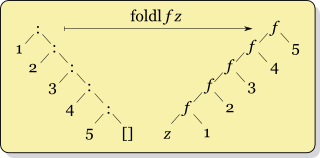
\includegraphics[height=0.30\textheight]{input_src/Left-fold-transformation.png} 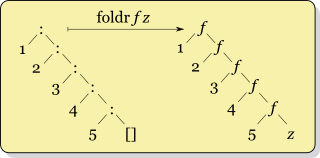
\includegraphics[height=0.30\textheight]{input_src/Right-fold-transformation.png}
	\end{center}
\end{frame}

\begin{frame}[fragile]
	\frametitle{Fold expression\titlehfill{}2/5}
	\begin{lstlisting}[language=C++]
template<typename... Args>
bool all(Args... args) { return (... && args); }

bool b = all(true, true, true, false);
// ((true && true) && true) && false\end{lstlisting}

	\begin{lstlisting}[language=C++]
template<typename... Args>
long long sum(Args... args) { return (args + ...); }

long long b = sum(1, 2, 3, 4);
// 1 + (2 + (3 + 4))\end{lstlisting}
\end{frame}

\begin{frame}[fragile]
	\frametitle{Fold expression\titlehfill{}3/5}
	
	\begin{alertblock}{\textit{left fold} ou \textit{right fold} ?}
	
	\begin{lstlisting}[language=C++]
template<typename... Args>
double div(Args... args) { return (... / args);}

div(1.0, 2.0, 3.0);      // 0.166667
// (1.0 / 2.0) / 3.0\end{lstlisting}

	\begin{lstlisting}[language=C++]
template<typename... Args>
double div(Args... args) { return (args / ...);}

div(1.0, 2.0, 3.0);      // 1.5
// 1.0 / (2.0 / 3.0)\end{lstlisting}
	\end{alertblock}
\end{frame}

\begin{frame}[fragile]
	\frametitle{Fold expression\titlehfill{}4/5}
	\begin{itemize}
		\item Si le \textit{parameter pack} est vide, le résultat est :
		\begin{itemize}
			\item \lstinline|true| pour l'opérateur \lstinline|&&|
			\item \lstinline|false| pour l'opérateur \lstinline||||
			\item \lstinline|void()| pour l'opérateur \lstinline|,|
		\end{itemize}
	\end{itemize}

	\begin{alertblock}{Attention}
		Un \textit{parameter pack} vide est une erreur pour les autres opérateurs
	\end{alertblock}
\end{frame}

\begin{frame}[fragile]
	\frametitle{Fold expression\titlehfill{}5/5}
	\begin{itemize}
		\item Compatible avec des opérateurs non arithmétiques ni logiques
	\end{itemize}

	\begin{lstlisting}[language=C++]
template<typename ...Args>
void FoldPrint(Args&&... args)
{ (cout << ... << forward<Args>(args)) << '\n';}

FoldPrint(10, 'a', "ert"s);\end{lstlisting}

	\begin{itemize}
		\item Y compris \og ,\fg{} qui va donner une séquence d'actions
	\end{itemize}

	\begin{lstlisting}[language=C++]
template<typename T, typename... Args>
void push_back_vec(std::vector<T>& v, Args&&... args)
{ (v.push_back(args), ...); }

vector<int> foo;
push_back_vec(foo, 10, 20, 56);\end{lstlisting}
\end{frame}

\subsection*{range-based for loop}
\begin{frame}[fragile]
	\frametitle{Contraintes de type \textit{range-based for loop}}
	\begin{itemize}
		\item Utilisation possible de types différents pour \lstinline|end| et \lstinline|begin|
		\item Permet de traiter des paires d'itérateurs
		\item \ldots{} mais aussi un itérateur et une taille
		\item \ldots{} ou un itérateur et une sentinelle de fin
		\item Compatible avec les travaux sur Range TS
		
\note[item]{Voir C++20 pour Range TS}
	\end{itemize}
\end{frame}

\subsection*{classe}
\begin{frame}[fragile]
	\frametitle{Modifications de l'héritage de constructeur}
	\begin{itemize}
		\item Constructeurs hérités visibles avec leurs paramètres par défaut

\note[item]{En C++11, les constructeurs avec paramètres par défaut (ou ellipses) étaient injectés en omettant valeurs par défaut (version avec le paramètre sans valeur par défaut et version sans le paramètre) et ellipse}

		\item Comportement identique aux autres fonctions héritées
	\end{itemize}

\note[item]{Le choix C++11 posait davantage de problèmes (pas de redéfinition avec valeur par défaut possible, multiples constructeurs par copie/déplacement, erreur de SFINAE, etc.)}

	\begin{alertblock}{Attention}
		Casse du code C++11 valide
	\end{alertblock}

	\begin{lstlisting}[language=C++]
struct Foo { Foo(int a, int b = 0); };
struct Bar : Foo 
{ Bar(int a); using Foo::Foo; };
struct Baz : Foo
{ Baz(int a, int b = 0); using Foo::Foo; };

Bar bar(0); // Ambigu (OK en C++11)
Baz baz(0); // OK (Ambigu en C++11)\end{lstlisting}

\note[item]{En C++11, Bar hérite de deux constructeurs - l'un avec deux paramètres int sans valeur par défaut et l'autre avec un paramètre int qui est surchargé par le constructeur de Bar}
\note[item]{En C++11, Baz hérite de deux constructeurs - l'un avec deux paramètres int sans valeur par défaut et l'autre avec un paramètre int - et défini un constructeur avec deux int dont un avec une valeur par défaut}

\note[item]{En C++17, Bar hérite d'un constructeur avec deux paramètres int dont une valeur par défaut et défini un constructeur avec un paramètre int}
\note[item]{En C++17, Baz  hérite d'un constructeur avec deux paramètres int dont un avec une valeur par défaut qu'il redéfini}
\end{frame}

\subsection*{Exception}
\begin{frame}[fragile]
	\frametitle{\lstinline|noexcept|}
	\begin{itemize}
		\item \lstinline|noexcept| fait partie du type des fonctions

		\begin{lstlisting}[language=C++]
void use_func(void (*func)() noexcept);
void my_func();

use_func(&my_func);       // Ne compile plus\end{lstlisting}

\note[item]{Une surcharge sans noexcept doit être ajoutée}

		\item Les fonctions \lstinline|noexcept| peuvent être convertie en fonctions non \lstinline|noexcept|
	\end{itemize}	

\end{frame}

\begin{frame}[fragile]
	\frametitle{\lstinline|std::uncaught_exceptions()|}
	\begin{itemize}
		\item \lstinline|std::uncaught_exceptions()| retourne le nombre d'exceptions lancées (ou relancées) et non encore attrapées du thread courant
	\end{itemize}

	\begin{lstlisting}[language=C++]
if(uncaught_exceptions())
{ ... }\end{lstlisting}

	\begin{block}{Motivation}
		Obtenir un comportement différent d'un destructeur en présence d'exception (p.ex. rollback)
	\end{block}
\end{frame}

\subsection*{Littéraux}
\begin{frame}[fragile]
	\frametitle{Caractères littéraux UTF-8}
	\begin{itemize}
		\item Écriture de caractère UTF-8 préfixé par \lstinline|u8|
		\item Lève une erreur si le caractère n'est pas représentable par un unique code point UTF-8
	\end{itemize}

	\begin{lstlisting}[language=C++]
char x = u8'x';\end{lstlisting}

\note[item]{Uniformisation avec les chaînes}
\end{frame}

\subsection*{Template}
\begin{frame}[fragile]
	\frametitle{Déduction de template dans les constructeurs\titlehfill{}1/3}
	\begin{itemize}
		\item Déduction des paramètres templates d'une classe à la construction
		\item Plus de déclaration explicite des paramètres template \ldots
		\item \ldots{}ni de \textit{make helpers}
	\end{itemize}

\note[item]{Généralisation de la déduction de paramètres template aux constructeurs}
\note[item]{Avant la déduction ne fonctionnait que pour les fonctions membres, pas pour les constructeurs}

	\begin{lstlisting}[language=C++]
pair<int, double> p(2, 4.5);
auto t = make_tuple(4, 3, 2.5);

// Devient

pair p(2, 4.5);
tuple t(4, 3, 2.5);\end{lstlisting}

\note[item]{Fonctionne avec \lstinline|pair p()|, \lstinline|pair p\{\}| et \lstinline|pair()| mais pas, pour l'instant, avec \lstinline|pair\{\}|}
\end{frame}

\begin{frame}[fragile]
	\frametitle{Déduction de template dans les constructeurs\titlehfill{}2/3}
	\begin{itemize}
		\item Permet de fournir une lambda en paramètre template sans la déclarer
	\end{itemize}

	\begin{lstlisting}[language=C++]
template<class Func> struct Foo { 
  Foo(Func f) : func(f) {} 
  Func func; };

Foo([&](int i) {...});\end{lstlisting}
\end{frame}

\begin{frame}[fragile]
\frametitle{Déduction de template dans les constructeurs\titlehfill{}3/3}
	\begin{block}{Note}
		Rend obsolète plusieurs \textit{make helper} (\lstinline|make_pair|, \lstinline|make_tuple|, etc.)
	\end{block}

	\begin{alertblock}{Attention}
		Ne permet pas la déduction partielle
		
		\begin{lstlisting}[language=C++]
std::tuple<int> t(1, 2, 3);  // Erreur\end{lstlisting}
	\end{alertblock}

\note[item]{Il faut donc fournir tous les paramètres templates ou aucun}
\end{frame}

\begin{frame}[fragile]
	\frametitle{\lstinline|template <auto>|}
	\begin{itemize}
		\item Déduction du type des paramètres templates numériques
	\end{itemize}

	\begin{lstlisting}[language=C++]
template <auto value> void foo() { }
foo<10>();  // int\end{lstlisting}

	\begin{lstlisting}[language=C++]
template <typename Type, Type value> 
  constexpr Type FOO = value;
constexpr auto const foo = FOO<int, 100>;

// Devient

template <auto value> constexpr auto FOO = value;
constexpr auto const foo = FOO<100>;
\end{lstlisting}

\end{frame}

\begin{frame}[fragile]
	\frametitle{Template \& contraintes d'utilisation\titlehfill{}1/2}
	\begin{itemize}
		\item typename autorisé dans les déclarations de template template parameters
	\end{itemize}

	\begin{lstlisting}[language=C++]
template <template <typename> typename C, typename T>
//                            ^^^^^^^^
   struct Foo { C<T> data; };

foo<std::vector, int> bar;\end{lstlisting}

\note[item]{Auparavant, il fallait obligatoirement utiliser class, alors que typename était valide partout ailleurs}
\end{frame}

\begin{frame}[fragile]
	\frametitle{Template \& contraintes d'utilisation\titlehfill{}2/2}
	\begin{itemize}
		\item Évaluation constante de tous les arguments templates \og non-types\fg{}
		\item Y compris pointeurs, références, pointeurs sur membres, \ldots
	\end{itemize}

	\begin{lstlisting}[language=C++]
template<int* P> struct Foo
{ int operator()() { return *P;} };
int N = 5;

Foo<&N> foo;     // OK
foo();           // 5

constexpr int* bar() { return &N; }
Foo<bar()> foo2; // OK
foo2();          // 5\end{lstlisting}
\end{frame}

\subsection*{Programmation fonctionnelle}
\begin{frame}[fragile]
	\frametitle{Capture de \lstinline|*this|}
	\begin{itemize}
		\item Capture \lstinline|*this| par valeur

\note[item]{Jusqu'à présent, on ne pouvait pas capturer la classe courante, seulement des attributs de celle-ci}
	\end{itemize}

	\begin{lstlisting}[language=C++]
[*this]() { ... }
[=, *this]() { ... }\end{lstlisting}

	\begin{lstlisting}[language=C++]
struct Foo {
  auto bar() {
    return [*this] { cout << s << endl; }; }

  std::string s; };

auto baz = Foo{"baz"}.bar();
baz();     // Affiche baz\end{lstlisting}
\end{frame}

\begin{frame}[fragile]
	\frametitle{Lambdas et expressions constantes\titlehfill{}1/3}
	\begin{itemize}
		\item Lambdas autorisées dans les expressions constantes \ldots
		\item \ldots{}si l'initialisation de chaque donnée capturée est possible dans l'expression constante
	\end{itemize}

	\begin{lstlisting}[language=C++]
constexpr int AddEleven(int n) {
  return [n] { return n+11; }();  }

AddEleven(5);   // 16\end{lstlisting}
\end{frame}

\begin{frame}[fragile]
	\frametitle{Lambdas et expressions constantes\titlehfill{}2/3}
	\begin{itemize}
		\item Déclaration \lstinline|constexpr| d'une lambda possible 
		\item Explicitement via \lstinline|constexpr|
	\end{itemize}

	\begin{lstlisting}[language=C++]
auto ID = [] (int n) constexpr { return n; };
constexpr int I = ID(3);\end{lstlisting}

	\begin{itemize}
		\item Implicitement \lstinline|constexpr| lorsque les exigences sont satisfaites
	\end{itemize}

\note[item]{Les lambdas sont donc \lstinline|constexpr| par défaut}

	\begin{lstlisting}[language=C++]
auto ID = [] (int n) { return n; };
constexpr int I = ID(3);\end{lstlisting}
\end{frame}

\begin{frame}[fragile]
	\frametitle{Lambdas et expressions constantes\titlehfill{}3/3}
	\begin{itemize}
		\item Fermeture de type littéral si les données sont des littéraux
	\end{itemize}

	\begin{lstlisting}[language=C++]
constexpr auto add = [] (int n, int m) {
  auto L = [=] { return n; };
  auto R = [=] { return m; };
  return [=] { return L() + R(); }; };

add(3, 4)()   // 7\end{lstlisting}
\end{frame}

\begin{frame}[fragile]
	\frametitle{\lstinline|std::invoke()|\titlehfill{}1/2}
	\begin{itemize}
		\item Appelle le \textit{callable} fourni en paramètre
		\item \ldots en fournissant la liste de paramètres
		\item \ldots et en retournant le retour du \textit{callable}
	\end{itemize}

	\begin{lstlisting}[language=C++]
int foo(int i) {
  return i + 42;}

invoke(&foo, 8);  // 50\end{lstlisting}
\end{frame}

\begin{frame}[fragile]
	\frametitle{\lstinline|std::invoke()|\titlehfill{}2/2}
	\begin{itemize}
		\item Fonctionne également avec des fonctions membres \ldots
		\item \ldots{} le premier paramètre fourni est l'objet à utiliser
	\end{itemize}

	\begin{lstlisting}[language=C++]
struct Foo {
  int bar(int i) {
    return i + 42; } };

Foo foo;
invoke(&Foo::bar, foo, 8);  // 50\end{lstlisting}

	\begin{block}{Motivation}
		Une syntaxe unique d'appel de \textit{callable}
	\end{block}
\end{frame}

\begin{frame}[fragile]
	\frametitle{\lstinline|std::not_fn()|}
	\begin{itemize}
		\item Construit un \textit{function object} en niant un appelable
	\end{itemize}

	\begin{lstlisting}[language=C++]
bool LessThan10(int a) 	{
  return a < 10; }
	
vector foo = { 1, 6, 3, 8, 14, 42, 2 };
count_if(begin(foo), end(foo), not_fn(LessThan10)); // 2\end{lstlisting}

	\begin{block}{Dépréciation}
		Dépréciation de \lstinline|std::not1| et \lstinline|std::not2|
	\end{block}
\end{frame}

\subsection*{Type traits}
\begin{frame}[fragile]
	\frametitle{Alias de traits}
	\begin{itemize}
		\item Ajout du suffixe \_v aux traits de la forme \lstinline|is_...|
		\item Suppression de \lstinline|::value|
	\end{itemize}

	\begin{lstlisting}[language=C++]
template <typename T>
enable_if_t<is_integral<T>::value, T>
sqrt(T t);

// Devient 

template <typename T>
enable_if_t<is_integral_v<T>, T>
sqrt(T t);\end{lstlisting}

\note[item]{Dans la continuité de \_t du C++14}

\end{frame}

\begin{frame}[fragile]
	\frametitle{Nouveaux traits}
	\begin{itemize}
		\item Nouveaux traits
		\begin{itemize}
			\item \lstinline|is_swappable_with|, \lstinline|is_swappable|, \lstinline|is_nothrow_swappable_with| et \lstinline|is_nothrow_swappable| : objets échangeables
			\item \lstinline|is_callable| et \lstinline|is_nothrow_callable| : objet appelable
			\item \lstinline|void_t| conversion en \lstinline|void|

\note[item]{Surtout utile en métaprogrammation via \lstinline|enable_if| et le SFINAE}

		\end{itemize}
		\item Méta-fonctions sur les traits
		\begin{itemize}
			\item \lstinline|std::conjunction| : \og ET\fg{} logique entre traits
			\item \lstinline|std::disjunction| : \og OU\fg{} logique entre traits
			\item \lstinline|std::negation| : négation d'un trait
		\end{itemize}

	\begin{lstlisting}[language=C++]
// foo disponible si tous ls Ts... ont le meme type
template<typename T, typename... Ts>
std::enable_if_t<std::conjunction_v<std::is_same<T, Ts>...>>
foo(T, Ts...) { }\end{lstlisting}
	\end{itemize}
\end{frame}

\subsection*{Attributs}
\begin{frame}[fragile]
	\frametitle{Gestion des attributs\titlehfill{}1/2}
	\begin{itemize}
		\item Usage étendu aux déclarations de \lstinline|namespace|
	\end{itemize}

	\begin{lstlisting}[language=C++]
namespace [[ Attribut ]] foo {}\end{lstlisting}

	\begin{itemize}
		\item Et aux valeurs d'une énumération
	\end{itemize}

	\begin{lstlisting}[language=C++]
enum foo {
  FOO_1 [[ Attribut ]],
  FOO_2 };\end{lstlisting}
\end{frame}

\begin{frame}[fragile]
	\frametitle{Gestion des attributs\titlehfill{}2/2}
	\begin{itemize}
		\item Attributs inconnus sont ignorés
	
\note[item]{Clarification de la norme, auparavant un compilateur pouvait lever une erreur car rien n'était précisé.}
\note[item]{Maintenant, il ne le peut plus et doit seulement ignorer l'attribut (éventuellement avec un avertissement).}

		\item \lstinline|Using| des attributs non standard
	\end{itemize}

	\begin{lstlisting}[language=C++]
[[ nsp::kernel, nsp::target(cpu,gpu) ]]
foo();

// Devient

[[ using nsp: kernel, target(cpu,gpu) ]]
foo();\end{lstlisting}
\end{frame}

\begin{frame}[fragile]
	\frametitle{Attribut \lstinline|[[ fallthrough ]]|}
	\begin{itemize}
		\item Placé dans un \lstinline|switch| avant un \lstinline|case| ou \lstinline|default|
		\item Indique qu'un cas se poursuit intentionnellement dans le cas suivant
		\item Incitation à ne pas lever de warning dans ce cas
	\end{itemize}

\note[item]{Remplace avantageusement de la duplication de code, des fonctions complétement \textit{ad hoc}, des désactivations abusives de warning (voire des warning ignorés), etc.}

	\begin{lstlisting}[language=C++]
switch(foo) {
  case 1:
  case 2:
    ...
[[ fallthrough ]];
  case 3:   // Idealement : pas de warning
    ...
  case 4:   // Idealement : warning
    ...
    break; }\end{lstlisting}

\note[item]{Les compilateurs offraient déjà des mécanismes similaires (\lstinline|__attribute__ ((fallthrough));| ou \lstinline|[[gnu::fallthrough]]| sur GCC, voire des commentaires à un format précis)}
\note[item]{Généralement pas de warning sur des case vides (cas 1-2 ici)}
\end{frame}

\begin{frame}[fragile]
	\frametitle{Attribut \lstinline|[[ nodiscard ]]|\titlehfill{}1/2}
	\begin{itemize}
		\item Indique que le retour d'une fonction ne devrait pas être ignorée
	\end{itemize}

	\begin{lstlisting}[language=C++]
[[ nodiscard ]] int foo() {return 5;}

foo();  // Idealement : warning\end{lstlisting}

	\begin{itemize}
		\item Incitation à lever un warning dans le cas contraire
	\end{itemize}

	\begin{block}{Note}
		Conversion implicite en \lstinline|void| pour supprimer le warning
		\begin{lstlisting}[language=C++]
(void)foo();\end{lstlisting}

\note[item]{Au moins avec gcc, à voir avec Visual et Clang} 
	\end{block}
\end{frame}

\begin{frame}[fragile]
	\frametitle{Attribut \lstinline|[[ nodiscard ]]|\titlehfill{}2/2}
	\begin{itemize}
		\item Possible sur la déclaration d'un type (classe, structure ou énumération)
		\item Indique qu'un retour de ce type ne devrait jamais être ignoré
	\end{itemize}

	\begin{lstlisting}[language=C++]
struct [[ nodiscard ]] Bar {};
Bar baz() { return Bar{}; }

baz();  // Idealement : warning\end{lstlisting}
\end{frame}

\begin{frame}[fragile]
	\frametitle{Attribut \lstinline|[[ maybe_unused ]]|\titlehfill{}1/2}
	\begin{itemize}
		\item Utilisable sur une classe, structure, fonction, variable, paramètre, \ldots
		\item Indique qu'un élément peut ne pas être utilisé
		\item Incitation à ne pas lever de warning en cas de non-utilisation
	\end{itemize}

	\begin{lstlisting}[language=C++]
[[ maybe_unused ]]
int foo([[ maybe_unused ]] int a,
        [[ maybe_unused ]] long b) {}\end{lstlisting}

	\begin{itemize}
		\item Ne devrait pas lever de warning en cas d'utilisation
	\end{itemize}
\end{frame}

\begin{frame}[fragile]
	\frametitle{Attribut \lstinline|[[ maybe_unused ]]|\titlehfill{}2/2}
	\begin{block}{Avant C++17}
		La méthode \og classique\fg{} pour supprimer le warning sur la non-utilisation de paramètres consiste à ne pas les nommer
		\begin{lstlisting}[language=C++]
int foo(int, long) {}\end{lstlisting}

\note[item]{Ce qui ne fonctionne pas très bien avec du code conditionnel sous option de compilation}
	\end{block}
\end{frame}

\begin{frame}[fragile]
	\frametitle{Attributs C++17 - Conclusion}
	\begin{exampleblock}{Do}
		Utilisez les attributs pour indiquer vos intentions

\note[item]{Au delà de l'information pour le compilateur et d'autres outils, c'est aussi une documentation à l'intention des relecteurs et correcteurs}
	\end{exampleblock}

	\begin{block}{Au delà du compilateur}
		Prise en compte par d'autres outils (générateurs de documentation, analyseurs statique de code) souhaitable
	\end{block}
\end{frame}

\subsection*{Multi-threading}
\begin{frame}[fragile]
	\frametitle{\lstinline|std::shared_mutex|}
	\begin{itemize}
		\item Similaire à \lstinline|std::mutex| avec deux niveaux d'accès
		\begin{itemize}
			\item Exclusif : possible si le verrou n'est pas pris
			\item Partagé : possible si le verrou n'est pas pris en exclusif
		\end{itemize}
		\item API identique à \lstinline|std::mutex| pour l'accès exclusif
		\item API similaire pour l'accès partagé
		\begin{itemize}
			\item \lstinline|lock_shared|
			\item \lstinline|try_lock_shared|
			\item \lstinline|unlock_shared|
		\end{itemize}
	\end{itemize}

	\begin{alertblock}{Attention}
		Un thread ne doit pas prendre un mutex qu'il possède déjà, même en accès partagé
	\end{alertblock}

	\begin{block}{Note}
		Équivalent non \og timed\fg{} de \lstinline|std::shared_timed_mutex|
	\end{block}
\end{frame}

\begin{frame}[fragile]
	\frametitle{\lstinline|std::scoped_lock|}
	\begin{itemize}
		\item \lstinline|std::scoped_lock| peut acquérir plusieurs mutex
	\end{itemize}

	\begin{lstlisting}[language=C++]
mutex first_mutex;
mutex second_mutex;

scoped_lock lck(first_mutex, second_mutex);\end{lstlisting}
\end{frame}

\subsection*{Library fundamentals TS}
\begin{frame}[fragile]
	\frametitle{\lstinline|std::apply()|}
	\begin{itemize}
		\item Appel de fonction depuis un tuple d'argument
	\end{itemize}

	\begin{lstlisting}[language=C++]
void foo(int a, long b, string c) {}

tuple bar{42, 5L, "bar"s};
apply(foo, bar);\end{lstlisting}

	\begin{itemize}
		\item Fonctionne sur tout ce qui supporte \lstinline|std::get()| et \lstinline|std::tuple_size|
		\item Notamment \lstinline|std::pair| et \lstinline|std::array|
	\end{itemize}

	\begin{lstlisting}[language=C++]
array<int, 3> baz{1, 54, 3};
apply(foo, baz);\end{lstlisting}

	\begin{itemize}
		\item De même, \lstinline|std::make_from_tuple()| permet de construire un objet depuis un \textit{tuple-like}
	\end{itemize}
\end{frame}

\begin{frame}[fragile]
	\frametitle{\lstinline|std::optional|\titlehfill{}1/4}
	\begin{itemize}
		\item Gestion d'objet dont la présence est optionnelle
		\item Issue de Boost.optional
		\item Interface similaire à un pointeur
		\begin{itemize}
			\item Testable via \lstinline|operator bool()|
			\item Accès à l'objet via \lstinline|operator*()|
			\item Accès au membre de l'objet via \lstinline|operator->()|

			\begin{alertblock}{Attention}
				L'appel de \lstinline|operator*()| ou \lstinline|operator->()| sur un \lstinline|std::optional| vide est indéfini
			\end{alertblock}

			\item \lstinline|std::nullopt| indique l'absence de l'objet
		\end{itemize}

		\item \lstinline|value()| retourne la valeur ou lève l'exception \lstinline|std::bad_optional_access|
		\item \lstinline|value_or()| retourne la valeur ou une valeur par défaut
	\end{itemize}
\end{frame}

\begin{frame}[fragile]
	\frametitle{\lstinline|std::optional|\titlehfill{}2/4}
	\begin{itemize}
		\item Supporte la déduction de type

	\begin{lstlisting}[language=C++]
optional foo(10);	// std::optional<int>\end{lstlisting}

		\item Supporte la construction \og en-place\fg{}
		
	\begin{lstlisting}[language=C++]
optional<complex<double>> foo{in_place, 3.0, 4.0};\end{lstlisting}
		
		\item \ldots Y compris depuis un \lstinline|std::initializer_list|
	\begin{lstlisting}[language=C++]
optional<vector<int>> foo(in_place, {1, 2, 3});\end{lstlisting}

		\item Existence du helper \lstinline|std::make_optional|
		
	\begin{lstlisting}[language=C++]
auto foo = make_optional(3.0);
auto bar = make_optional<complex<double>>(3.0, 4.0);\end{lstlisting}
	\end{itemize}
\end{frame}

\begin{frame}[fragile]
	\frametitle{\lstinline|std::optional|\titlehfill{}3/4}
	\begin{itemize}
		\item Changement de la valeur via \lstinline|reset|, \lstinline|swap|, \lstinline|emplace| ou \lstinline|operator=()|
		\item Comparaison naturelle des valeurs contenues 

		\begin{lstlisting}[language=C++]
optional<int> deux(2), dix(10);

dix > deux;   // true	
dix < deux;   // false
dix == 10;    // true\end{lstlisting}

		\item \ldots En prenant en compte \lstinline|std::nullopt|

		\begin{lstlisting}[language=C++]
optional<int> none, dix(10);

dix > none;       // true	
dix < none;       // false
none == 10;       // false
none == nullopt;  // true\end{lstlisting}
	\end{itemize}
\end{frame}

\begin{frame}[fragile]
	\frametitle{\lstinline|std::optional|\titlehfill{}4/4}
	\begin{alertblock}{\lstinline|std::optional<bool>| et \lstinline|std::optional<T*>|}
		Probablement plus pertinent d'utiliser :
		\begin{itemize}
			\item Des booléens \og trois états\fg{} (Boost.tribool)
			\item Des pointeurs bruts
		\end{itemize}
	\end{alertblock}

	\begin{exampleblock}{Do}
		Préférez \lstinline|optional| aux pointeurs bruts pour gérer des données optionnelles

\note[item]{Sémantique plus précise, pas de risque de tentative de libération ou de fuite mémoire, \lstinline|value()| et \lstinline|value_or()| permettent de simplifier l'usage}
	\end{exampleblock}

	\begin{block}{En attendant C++17 \ldots}
		Utilisez Boost.Optional
	\end{block}
\end{frame}

\begin{frame}[fragile]
	\frametitle{\lstinline|std::any|\titlehfill{}1/4}
	\begin{itemize}
		\item \lstinline|void*| \textit{type-safe} contenant un objet de n'importe quel type (ou vide)
		\item Implémentation de \textit{Type-erasure}
		
\note[item]{Pour les données, tout comme \lstinline|std::function| est un \textit{type-erasure} pour les appelables}
		
		\item Introduction d'une forme de \og typage dynamique\fg{} au sein de C++

\note[item]{Ce n'est pas réellement du typage dynamique : ce n'est pas dans le langage mais une classe \textit{type-erasure} dans la bibliothèque standard et les instances restent typées statiquement avec le type \lstinline|std::any| mais en terme d'utilisation ça rend un service équivalent}

		\item Issue de Boost.Any
		\item Type contenu dépend de la valeur assignée

	\begin{lstlisting}[language=C++]
any a = 1;  // int
a = 3.14;   // double
a = true;   // bool\end{lstlisting}
	\end{itemize}
\end{frame}

\begin{frame}[fragile]
	\frametitle{\lstinline|std::any|\titlehfill{}2/4}
	\begin{itemize}
		\item Supporte la construction \og en-place\fg{}

			\begin{lstlisting}[language=C++]
any a(in_place_type<complex<double>>, 3.0, 4.0);\end{lstlisting}

		\item Existence du \textit{helper} \lstinline|std::make_any|

			\begin{lstlisting}[language=C++]
any a = make_any<complex<double>>(3.0, 4.0);\end{lstlisting}

		\item Changement de valeur (et éventuellement de type) via l'affectation

			\begin{lstlisting}[language=C++]
std::any a = 1;
a = 3.14;
\end{lstlisting}
	
		\item \ldots ou \lstinline|emplace()|
			\begin{lstlisting}[language=C++]
a.emplace<std::complex<double>>(3.0, 4.0);
\end{lstlisting}

	\end{itemize}
\end{frame}

\begin{frame}[fragile]
	\frametitle{\lstinline|std::any|\titlehfill{}3/4}
	\begin{itemize}
		\item \lstinline|any_cast<Type>()| récupère la valeur \ldots
		\item \ldots{} et lève une exception si le type demandé n'est pas correct

		\begin{lstlisting}[language=C++]
any a = 1;
any_cast<int>(a);  // 1
any_cast<bool>(a); // Lance bad_any_cast\end{lstlisting}

		\item ou récupère l'adresse \ldots
		\item \ldots{} et retourne \lstinline|nullptr| si le type demandé n'est pas correct

		\begin{lstlisting}[language=C++]
any a = 1;
int* foo = any_cast<int>(&a);
int* foo = any_cast<bool>(&a);     // nullptr\end{lstlisting}
	\end{itemize}
\end{frame}

\begin{frame}[fragile]
	\frametitle{\lstinline|std::any|\titlehfill{}4/4}
	\begin{itemize}
		\item \lstinline|reset()| vide le contenu
		\item \lstinline|has_value()| teste la vacuité
		\item \lstinline|type()| récupère l'information du type courant
	\end{itemize}

	\begin{block}{En attendant C++17 \ldots}
		Utilisez Boost.Any
	\end{block}
\end{frame}

\begin{frame}[fragile]
	\frametitle{\lstinline|std::string_view|\titlehfill{}1/3}
	\begin{itemize}
		\item \lstinline|std::basic_string_view| référence une séquence contiguë de caractères
		\item Quatre spécialisations standard (une pour chaque type de caractère)

\note[item]{Soit \lstinline|char|, \lstinline|wchar|, \lstinline|char16_t| et \lstinline|char32_t|}

		\item Référence non possédante sur une séquence pré-existante
		\item Pas de modification de la séquence depuis la vue
	\end{itemize}

	\begin{alertblock}{Attention !}
		\begin{itemize}
			\item Pas de \lstinline|\0| terminal systématique
			\item La chaîne référencée doit vivre au moins aussi longtemps que la vue
		\end{itemize}
	\end{alertblock}
\end{frame}

\begin{frame}[fragile]
	\frametitle{\lstinline|std::string_view|\titlehfill{}2/3}
	\begin{itemize}
		\item Accès aux caractères : \lstinline|operator[]()|, \lstinline|at()|, \lstinline|front()|, \lstinline|back()|, \lstinline|data()|
		\item Modification des bornes : \lstinline|remove_prefix()| et \lstinline|remove_suffix()|
		\item Accès à la taille et à la taille maximale : \lstinline|size()|, \lstinline|length()| et \lstinline|max_size()|
		\item Test de vacuité : \lstinline|empty()|
		\item Construction d'une chaîne depuis la vue : \lstinline|to_string()|
		\item Copie d'une partie de la vue : \lstinline|copy()|
		\item Construction d'une vue sur une sous-partie de la vue : \lstinline|substr()|
		\item Comparaison avec une autre vue ou une chaîne : \lstinline|compare()|
		\item Recherche : \lstinline|find()|, \lstinline|rfind()|, \lstinline|find_first_of()|, \lstinline|find_last_of()|, \lstinline|find_first_not_of()|, \lstinline|find_last_not_of|
		\item Comparaison lexicographique : \lstinline|==|, \lstinline|!=|, \lstinline|<=|, \lstinline|>=|, \lstinline|<| et \lstinline|>|
		\item Affichage : \lstinline|operator<<()|
	\end{itemize}
\end{frame}

\begin{frame}[fragile]
	\frametitle{\lstinline|std::string_view|\titlehfill{}3/3}
	\begin{lstlisting}[language=C++]
string foo = "Lorem ipsum dolor sit amet";

string_view bar(&foo[0], 11);
cout << bar.size() << " - " << bar << '\n';
// 11 - Lorem ipsum

bar.remove_suffix(6);
cout << bar.size() << " - " << bar << '\n';
// 5 - Lorem\end{lstlisting}

	\begin{exampleblock}{Performances}
		\begin{itemize}
			\item Souvent meilleures que les fonctionnalités équivalentes de \lstinline|string| \ldots
			\item \ldots{} mais pas toujours, donc mesurez
		\end{itemize} 

\note[item]{Et que boost.split}
\note[item]{Notamment car il y a moins d'allocation mémoire}
\note[item]{La contrepartie c'est qu'il n'y a pas de chaîne de construite ni de modification possible}
\note[item]{Travailler à base de chaîne peut être plus rapide lorsque le compilateur peut optimiser correctement le code avec les chaîne, si on construit une chaîne au final p.ex.}
	\end{exampleblock}
\end{frame}

\begin{frame}[fragile]
	\frametitle{Mémoire}
	\begin{itemize}
		\item \lstinline|std::shared_ptr| et \lstinline|std::weak_ptr| sur des tableaux

	\begin{lstlisting}[language=C++]
std::shared_ptr<int[]> foo(new int[10]);\end{lstlisting}

\begin{alertblock}{Pas de \lstinline|std::make_shared()|}
	\lstinline|std::make_shared()| ne supporte pas les tableaux en C++17
\end{alertblock}

		\item Évolutions des allocateurs

\note[item]{\textit{Type-erased allocator}, \textit{polymorphic allocator}, \textit{memory ressources}}
\note[item]{Gestion de l'alignement des \textit{Over-Aligned Data}}

		\item Classe de gestion de pools de ressources (synchronisés ou non)
	\end{itemize}

	\begin{block}{Note}
		Présence dans le TS d'un pointeur intelligent sans responsabilité (observateur) : \lstinline|observer_ptr|, mais n'est pas dans le périmètre accepté pour C++17
	\end{block}
\end{frame}

\begin{frame}[fragile]
	\frametitle{Algorithmes}
	\begin{itemize}
		\item Recherche d'une séquence dans une autre
		\begin{itemize}
			\item Trois foncteurs de recherche : default, Boyer-Moore et Boyer-Moore-Horspoll
			\item \lstinline|std::search()| encapsule l'appel à un des foncteurs
		\end{itemize}
		\item Échantillonnage
		\begin{itemize}
			\item \lstinline|std::sample()| extrait aléatoirement n éléments d'un ensemble
		\end{itemize}
	\end{itemize}

	\begin{lstlisting}[language=C++]
string in = "abcdefgh", out;
sample(begin(in), end(in), back_inserter(out), 
       5, mt19937{random_device{}()});\end{lstlisting}
\end{frame}

\begin{frame}[fragile]
	\frametitle{PGCD et PPCM}
	\begin{itemize}
		\item Ajout des fonctions \lstinline|gcd| et \lstinline|lcm|
		\item Initialement prévu pour des versions ultérieures \ldots
		\item \ldots mais suffisamment simples et élémentaires pour C++17 
	\end{itemize}

	\begin{lstlisting}[language=C++]
gcd(12, 18);   // 6
lcm(12, 18);   // 36\end{lstlisting}
\end{frame}

\subsection*{Filesystem TS}
\begin{frame}[fragile]
	\frametitle{\textit{Filesystem} TS\titlehfill{}1/3}
	\begin{itemize}
		\item Gestion des systèmes de fichiers
		\item Adapté à l'OS et au système de fichiers utilisés
		\item Issue de Boost.Filesystem
		\item Manipulation des chemins et noms de fichiers
	\end{itemize}

	\begin{lstlisting}[language=C++]
path foo("/home/foo");
path bar(foo / "bar.txt");
bar.filename();    // bar.txt
bar.extension();   // .txt
bar.native();      // std::string
bar.c_str();       // const char*\end{lstlisting}
\end{frame}

\begin{frame}[fragile]
	\frametitle{\textit{Filesystem} TS\titlehfill{}2/3}
	\begin{itemize}
		\item Manipulation des répertoires, des fichiers et de leurs métadatas
		\begin{itemize}
			\item Copie : \lstinline|copy_file()|, \lstinline|copy()|
			\item Création de répertoires : \lstinline|create_directory()|, \lstinline|create_directories()|

\note[item]{Différence : création du répertoire final seulement ou de tous les répertoires intermédiaires nécessaires}

			\item Création des liens : \lstinline|create_symlink()|, \lstinline|create_hard_link()|
			\item Test d'existence : \lstinline|exists()|
			\item Taille : \lstinline|file_size()|
			\item Type : \lstinline|is_regular_file()|, \lstinline|is_directory|, \lstinline|is_symlink()|, \lstinline|is_fifo()|, \lstinline|is_socket()|, \ldots
			\item Permissions : \lstinline|permissions()|
			\item Date de dernière écriture : \lstinline|last_write_time()|
			\item Suppression : \lstinline|remove()|, \lstinline|remove_all()|

\note[item]{Différence \lstinline|remove| et \lstinline|remove_all| : suppression récursive pour le second}

			\item Changement de nom : \lstinline|rename()|
			\item Changement de taille : \lstinline|resize_file()|
			\item Chemin du répertoire temporaire : \lstinline|temp_directory_path()|
			\item Chemin du répertoire courant : \lstinline|current_path()|
		\end{itemize}
	\end{itemize}
\end{frame}

\begin{frame}[fragile]
	\frametitle{\textit{Filesystem} TS\titlehfill{}3/3}
	\begin{itemize}
		\item Parcours de répertoires
		\begin{itemize}
			\item Entrée du répertoire : \lstinline|directory_entry|
			\item Itérateurs pour le parcours
			\begin{itemize}
				\item Parcours simple : \lstinline|directory_iterator|
				\item Parcours récursif : \lstinline|recursive_directory_iterator|
			\end{itemize}
			\item Construction de l'itérateur de début depuis le chemin du répertoire
			\item Construction de l'itérateur de fin par défaut
		\end{itemize}
		\item \lstinline|std::fstream| constructible depuis \lstinline|path|
	\end{itemize}

	\begin{exampleblock}{Do}
		Utilisez \textit{Filesystem} plutôt que les API C ou systèmes
	\end{exampleblock}

	\begin{block}{En attendant C++17 \ldots}
		Utilisez Boost.Filesystem

\note[item]{Ou Qt, POCO, etc. L'idée est d'avoir un code portable, mieux typé et moins source d'erreur}
\note[item]{Préférence pour Boost car proche de ce que sera std}
	\end{block}
\end{frame}

\subsection*{Parallelism TS}
\begin{frame}[fragile]
	\frametitle{\textit{Parallelism} TS\titlehfill{}1/5}
	\begin{itemize}
		\item Ajout de surcharges \og parallèles\fg{} à de nombreux algorithmes standard
		\item Politiques d'exécution (séquentielle, parallèle et parallèle+vectorisée)
	\end{itemize}

	\begin{lstlisting}[language=C++]
void bar(int i);

vector<int> foo {0, 5, 42, 58};
for_each(execution::par, begin(foo), end(foo), bar);\end{lstlisting}

	\begin{alertblock}{Attention}
		Accès concurrents non gérés intrinsèquement par l'exécution parallèle\\
		Responsabilité du développeur de choisir des structures de données et des foncteurs adressant ce point
	\end{alertblock}
\end{frame}

\begin{frame}[fragile]
	\frametitle{\textit{Parallelism} TS\titlehfill{}2/5}
	\begin{itemize}
		\item \lstinline|std::for_each_n()| : variante de \lstinline|std::for_each()| prenant l'itérateur de début et une taille et non une paire d'itérateurs

\note[item]{En soi, ce n'est pas lié au parallélisme mais cet algorithme apparait avec ce TS}

		\item \lstinline|std::reduce()| \og ajoute\fg{} tous les éléments de l'ensemble
	\end{itemize}

	\begin{block}{\lstinline|std::reduce()| ou \lstinline|std::accumulate()| ?}
		L'ordre des \og additions\fg{} n'est pas spécifié dans le cas de \lstinline|std::reduce()|

\note[item]{Le résultat n'est donc pas déterministe dans le cas d'opérations non associatives ou non commutatives (car \lstinline|std::reduce()| regroupe et réarrange les opérations)}
\note[item]{Mais rend cet algorithme parallélisable contrairement à \lstinline|std::accumulate()|}
	\end{block}
\end{frame}

\begin{frame}[fragile]
	\frametitle{\textit{Parallelism} TS\titlehfill{}3/5}
	\begin{itemize}
		\item \lstinline|std::exclusive_scan()| construit un ensemble où chaque élément est égal à la somme des éléments de rang strictement inférieur de l'ensemble initial et d'une valeur initiale
	\end{itemize}

	\begin{lstlisting}[language=C++]
vector<int> foo {5, 42, 58}, bar;

exclusive_scan(begin(foo), end(foo), 
               back_inserter(bar), 8);
// bar : 8 13 55\end{lstlisting}
\end{frame}

\begin{frame}[fragile]
	\frametitle{\textit{Parallelism} TS\titlehfill{}4/5}
	\begin{itemize}
		\item \lstinline|std::inclusive_scan()| construit un ensemble où chaque élément est égal à la somme des éléments de rang inférieur ou égal de l'ensemble initial et d'une valeur initiale (si présente)
	\end{itemize}

	\begin{lstlisting}[language=C++]
vector<int> foo {5, 42, 58};
vector<int> bar;

inclusive_scan(begin(foo), end(foo), 
               back_inserter(bar), 8);
// bar : 13 55 113\end{lstlisting}

\note[item]{\lstinline|exclusive_scan| et \lstinline|inclusive_scan| sont proche de \lstinline|partial_sum| mais sans garanti d'ordre des \og additions\fg{} avec résultat indéterminé en cas d'opérations non associatives (idem \lstinline|reduce()| / \lstinline|accumulate()|)}
\end{frame}

\begin{frame}[fragile]
	\frametitle{\textit{Parallelism} TS\titlehfill{}5/5}
	\begin{itemize}
		\item \lstinline|std::transform_reduce()| : \lstinline|std::reduce()| sur des éléments préalablement transformés
		\item \lstinline|std::transform_exclusive_scan()| : \lstinline|std::exclusive_scan()| sur des éléments préalablement transformés
		\item \lstinline|std::transform_inclusive_scan()| : \lstinline|std::inclusive_scan()| sur des éléments préalablement transformés
	\end{itemize}

	\begin{block}{Note}
		La transformation n'est pas appliquée à la graine
	\end{block}
\end{frame}

\subsection*{Mathematical Special Functions}
\begin{frame}[fragile]
	\frametitle{\textit{Mathematical Special Functions}}
	\begin{itemize}
		\item Une longue histoire datant du TR1
		\item Ajout de fonctions mathématiques particulières :
		\begin{itemize}
			\item Fonctions cylindriques de Bessel
			\item Fonctions de Neumann
			\item Polynômes de Legendre
			\item Polynômes de Hermite
			\item Polynômes de Laguerre
			\item \ldots
		\end{itemize}
	\end{itemize}
\end{frame}
\end{document}